\section{Introduciton to analysis of optimisation}
\label{sec:introduction to analysis of optimisation}
In optimizing algorithms we need to first understand where the time is being spend and afterwards analyse how much we are able to speed up this process with.
In understanding the problem and bottlenecks we utilize the profiling tools by nvidia called ``nvprof'', elaborated in \cref{sec:profiling}.
For analysing purposes we approach the problem from two perspectives, a theoretical based, in \cref{sec:amdahls law} on understanding the relationship between parallizability and number of cores and a more hardware specific, elaborated in \cref{sec:analysing hardware}, where we analyse theoretical memory bandwidth usage.
Hardware-wise the bottleneck is often to read/write to global memory.
As many of our tasks are relatively simple and does not require much computation we will only consider theoretical memory bandwidth as a concrete performance measure.

\subsection{Profilling}
\label{sec:profiling}
To understand our problem from a runtime perspective we must quantify the execution time in ``metrics'' of the different ``events'' in our program.
An event is some quantifiable activity, action, or occurrence on a GPGPU device.
Metrics are a set of runtime descriptions of one or more events.i

In order to gather metrics about our events we utilize the built-in CUDA tool \ttt{nvprof}, which is a command-line debugging tool to profile compiled CUDA code.
The property of being a command-line tool makes \ttt{nvprof} especially usefull for us as we are limited to executing code on remote servers.

By default \ttt{nvprof} gives a short summary of how much time was spent on the different invocations.
The default settings shows where time is spent throughout the application.
The debugger is invoked as follows
%
\begin{quote}
  \ttt{nvprof [options] [CUDA-application] [application-arguments]}
\end{quote}
%
To give a detailed metrics description the flag \ttt{--print-gpu-trace} can be utilized, this flag will print a list of all kernel invocations.
Further \ttt{--print.gpu-trace} will show metrics such as the amount of memory used, where it is used, what the memory's transfer rate was, on which GPGPU the kernel ran, the execution time, etc.~\cite{profiling2015doc}
Aside from writing its results to the terminal it is also possible to write the profiling results to a file.
Furthermore, to gain insight into opportunities for optimisation the \ttt{--analysis-metrics} flag allows nvprof to capture statistics for analysis of the GPGPU's metrics.
These statistics can be used with Nvidia's visual profiler to perform a ``guided analysis'' which we utilizes in \todo{nvvp fast histo!}.~\cite{nvprof2013tips}

\subsection{Strong scaling - Amdahl's Law}
\label{sec:amdahls law}

Amdahl's Law approximates the potential speed up of a serial program.
The equation is presented in \cref{eq:amdahls law}, where $P$ is the portion of the serial code that can be parallelized, $(1-P)$ is the portion that cannot be parallelized and $n$ is the amount of processors available.
Thus, $S(n)$ is the theoretical speed up achievable while holding the workload constant.

\begin{equation}
  \label{eq:amdahls law}
  S(n) = \frac{1}{(1-P) + P/n}
\end{equation}

Amdahl's Law only applies if the amount of work performed in the parallel version is not significantly different than the serial code's amount of work.
An illustration of the potential speed up is presented in \cref{fig:amdahls law} with $n=1024$.
The model thus theorize that given a fully parallizable problem, the problem should be executed $n$ times faster~\cite{farber2011cuda}.

\begin{figure}[htb]
  \centering
  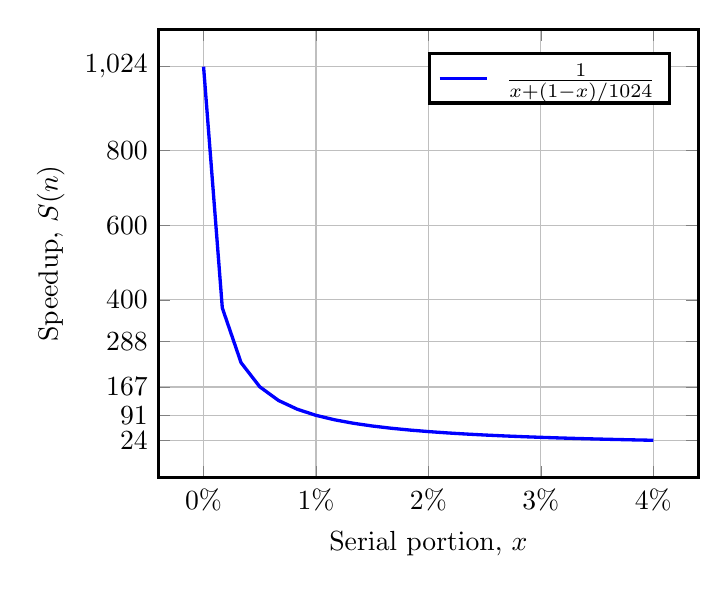
\begin{tikzpicture}
  \begin{axis}[
    ymajorgrids,
    xmajorgrids,
    ylabel={Speedup, $S(n)$},
    ytick={24,91,167,288,400,600,800,1024},
    xlabel={Serial portion, $x$},
    scaled x ticks = false, % do not add axis-multiplier
    xticklabel={% print percent
      \pgfmathparse{\tick*100}%
      \pgfmathprintnumber{\pgfmathresult}%
      \%%
    },
    legend style={
      at={(0.95,0.95)},
      anchor=north east,
      column sep=1ex
     },
     no markers,
     very thick
  ]

  \addplot+[domain=0.00:0.04] {1/(x+((1-x)/1024))};
  \addlegendentry{$\frac{1}{x + (1-x) / 1024}$};
  \end{axis}
\end{tikzpicture}

  \caption{Speed up by Amdahl's Law, where $x=(1-P)$, $(1-x)=P$, and $n=1024$}
  \label{fig:amdahls law}
\end{figure}

An important property of Amdahls is the decline of the curve as the solution moves from 0\% to 1\%.
With parallel portion $P=0.99$ the speed up is approximately $91\times$, and $1024\times$ when $P=1.00$ and everything can be executed in parallel.
According to Amdahl's Law, with just a tiny portion of the code that cannot be executed in parallel, a high speed up is not likely to be achieved.

\todo{in section xyz we use this to analyse a problem statement}

\subsection{Gustafson-Barsis Law}
\label{sec:gustafson-barsis law}

Gustafson and Barsis Law approximates how much more throughput can be achieved by increasing processor count given a constant amount of time.
This type of formulation is often interesting when computing problems that are open ended such as computing pi -- given more computational power, the processors can compute more digits of pi in the same time~\cite{amdahlorgustafson2011}.

\begin{equation}
  \label{eq:gustafson-barsis law}
  W(n) = n + (1-n) \times (1-P)
\end{equation}
Where $P$ is the amount of the program that can be parallelized and $W(n)$ is the theoretical increase in throughput over a defined period of time.~\cite{gustafson1988reevaluating}.

\todo{Fuck gustav?}

\subsection{Theoretical memory speed-up}
\label{sec:analysing hardware}
In order to access the usage of the theoretical memory bandwitdth in our optimization we can use the hardware specific numbers to see how much data we should be able to push through the GPGPU.
We need to find the clock rate to determine how fast the processesors are running and the bus width to determine the amount of data transfered at every clock multiplied by 2 due to double data rate.\footnote{http://devblogs.nvidia.com/parallelforall/how-implement-performance-metrics-cuda-cc/}
The formulation for theoretical memory bandwidth thus becomes:
\begin{equation*}
output \frac{bytes}{s} = \frac{clock}{sec} * \frac{bytes}{clock} * 2
\end{equation*}
Reading out \ttt{deviceQuery} information \cref{aap:tesla k40 specifications} we can access that the \ttt{Memory Clock Rate: 3004 Mhz} and \ttt{Memory Bus Width: 384}.
Thus out theoretical memory bandwidth on out K40 is
\begin{equation*}
288.384 \frac{GB}{s} = 3.004 Ghz * 48 \frac{bytes}{clock} * 2
\end{equation*}
In order to understand how close our solution is to the theoretical memory bandwidthwe use the following formula:
\begin{equation*}
percentage of theoretical = \frac{\frac{read/writes in GBs}{time in seconds}}{288.384} * 100
\end{equation*}
In \todo{cref section} we use this tool to analyse a problem statement.
